\documentclass[12pt,letterpaper]{article}

\usepackage[utf8]{inputenc}
\usepackage[T1]{fontenc}
\usepackage{amsmath}
\usepackage{amsfonts}
\usepackage{amssymb}
\usepackage{amsthm}
\usepackage[left=2cm,right=2cm,top=2cm,bottom=2cm,headheight=22pt]{geometry}
\usepackage{fancyhdr}
\usepackage{setspace}
\usepackage{lastpage}
\usepackage{graphicx}
\usepackage{caption}
\usepackage{subcaption}
\usepackage{paralist}
\usepackage{url}

\theoremstyle{definition}
\newtheorem{question}{Question}
\newtheorem{example}{Example}
\newtheorem{exercise}[question]{Exercise}
\newtheorem*{challenge}{Challenge}
\newtheorem*{theorem}{Theorem}
\newtheorem*{definition}{Definition}

\begin{document}

%Paramètres de mise en forme des paragraphes selon les normes françaises
\setlength{\parskip}{1ex plus 0.5ex minus 0.2ex}
\setlength{\parindent}{0pt}

%Paramètres relatifs aux en-têtes et pieds de page.
\pagestyle{fancy}
\lhead{Theron J Hitchman}
\chead{\Large Reading and Guided Practice \#12}
\rhead{Fall 2013}
\lfoot{\emph{Math and Decision Making}}
\cfoot{}
\rfoot{\emph{\thepage\ of \pageref{LastPage}}}

\section*{Introduction}
This reading is about a numerical invariant for knots, called the \emph{unknotting number}.

\section*{Goals}
At the end of this assignment, a student should be able to:
\begin{compactitem}
\item Describe a method for changing crossings that will unknot any knot, and explain why it works.
\item Compute the unknotting number for knots with a small number of crossings.
\item Explain why computing unknotting number is challenging in general.
\end{compactitem}
A student might also be able to:
\begin{compactitem}
\item Solve an open problem about unknotting numbers.
\end{compactitem}

\section*{Reading and Questions for 25 September}

\begin{theorem}
Let $K$ be a knot.
By changing some subset of the crossings, it is possible to change $K$ into the unknot.
\end{theorem}

Here is a recipe for doing this.
Pick a point $P$ on the knot, and some direction of travel away from $P$.
As you ``walk along the knot,'' each time you reach a new crossing and are travelling on the understrand through that crossing, change the roles of understrand and overstrand.
If you reach a crossing you have been through before, or if you reach a new crossing first by taking an overstrand, leave that crossing alone.
The process stops when you reach $P$ again.

Here is an example of the process in action with the knot $8_20$.

\begin{figure}[h]
    \centering
    \begin{subfigure}{.3\textwidth}
        \centering
        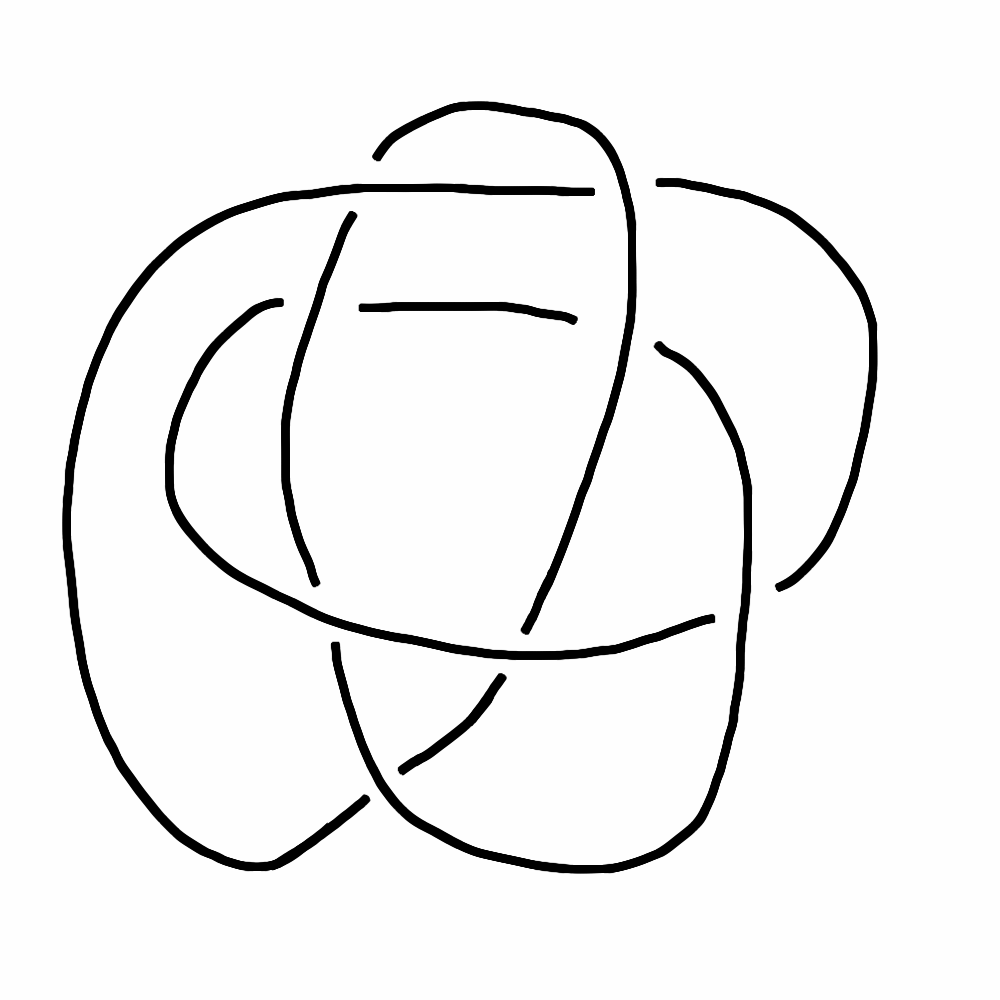
\includegraphics[width=\textwidth]{rgp12pics/8-20.png}
        \caption{The knot $8_{20}$.}
    \end{subfigure}
    \begin{subfigure}{.3\textwidth}
        \centering
        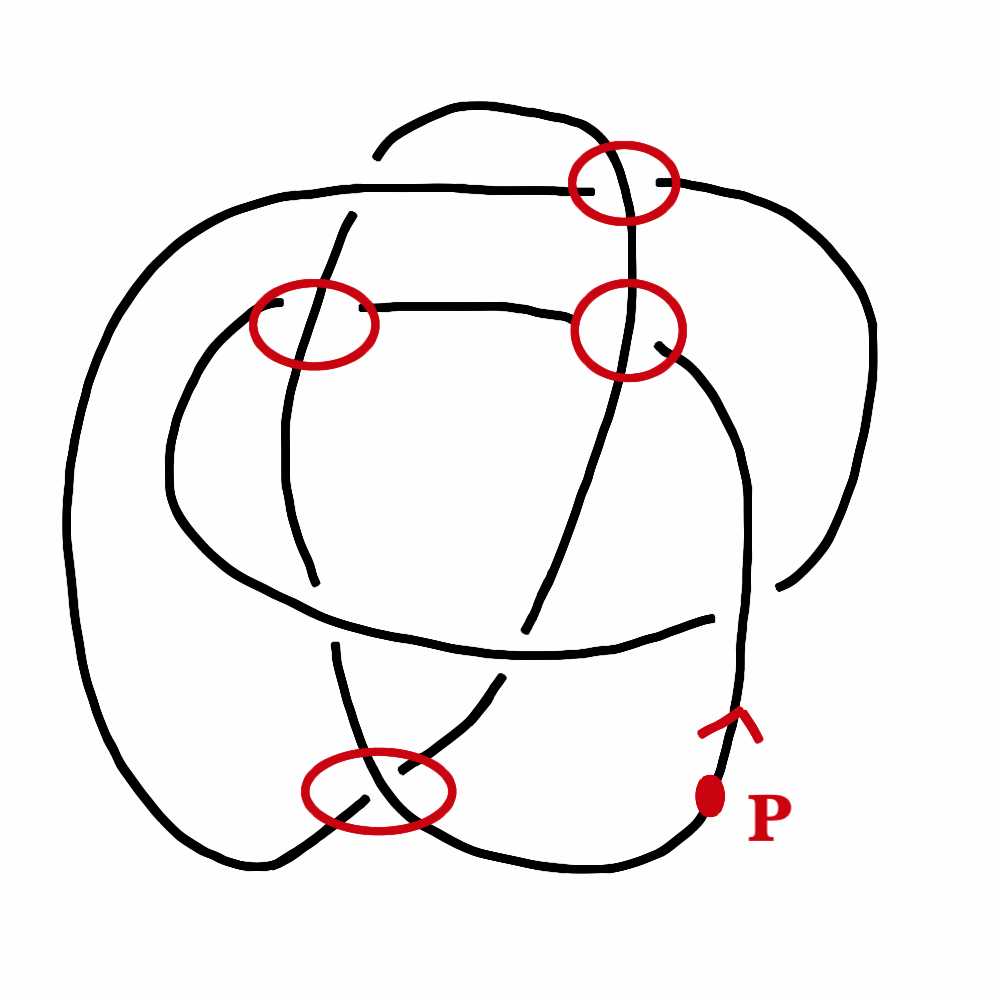
\includegraphics[width=\textwidth]{rgp12pics/8-20-changes.png}
        \caption{The knot $8_{20}$ with spots for changes labeled.}
    \end{subfigure}
    \begin{subfigure}{.3\textwidth}
        \centering
        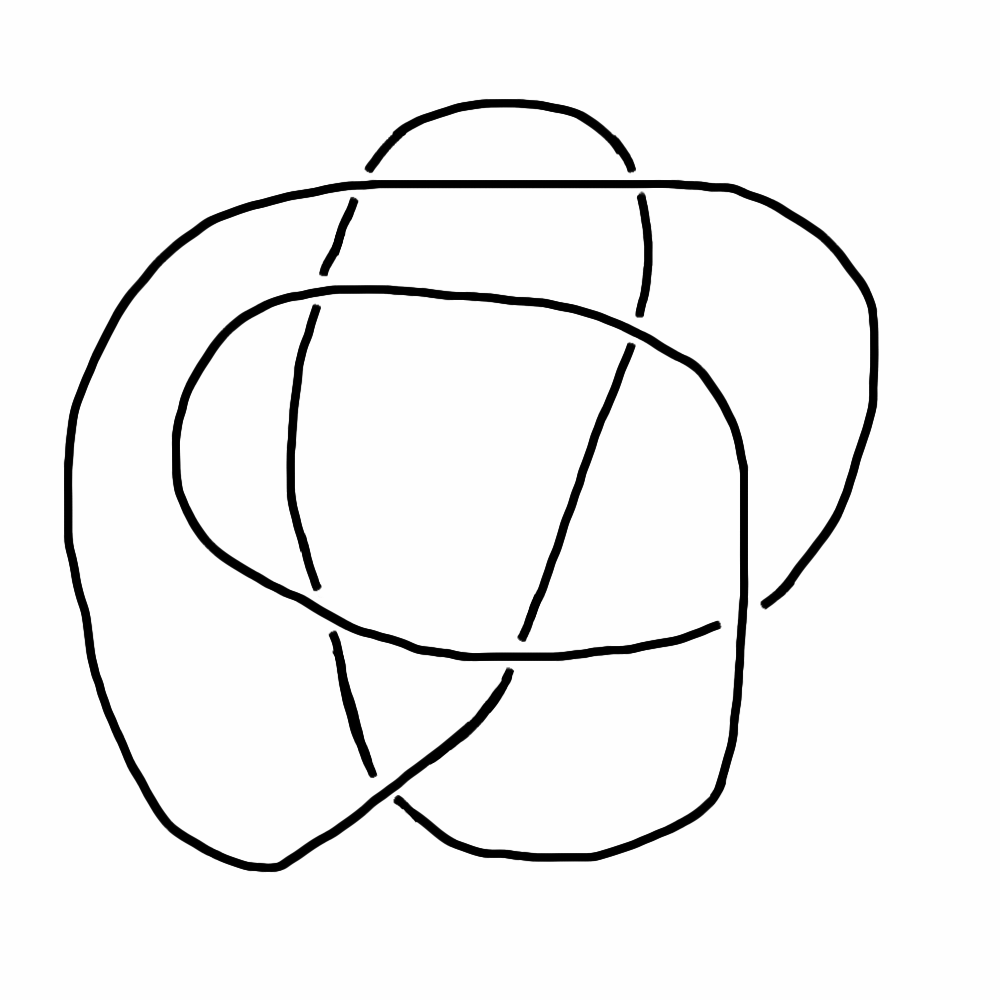
\includegraphics[width=\textwidth]{rgp12pics/8-20-unknot.png}
        \caption{The unknot.}
    \end{subfigure}
\end{figure}

\clearpage

\begin{exercise}
Try the process yourself on the trefoil knot.
\end{exercise}

\begin{figure}[h]
    \centering
    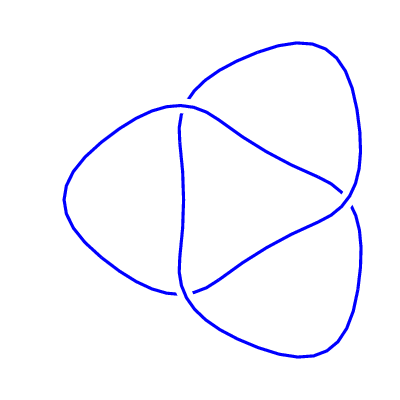
\includegraphics[width=.4\textwidth]{rgp12pics/3_1.png}
    \caption{The trefoil knot}
\end{figure}

This process is enough to prove the theorem, because it \emph{always} works.
That is, after following this process, you will always end up with the unknot.

\begin{challenge}
Why does that process always work?
\end{challenge}


\section*{The Unknotting Number of a Knot}

The theorem we just explored allows us to make a definition of a new invariant. This invariant will be a number, much like linking number for links, but it will only work for knots.

\begin{definition}
Let $K$ be a knot.
The \emph{unknotting number} of $K$ is the smallest number, $u(K)$, of crossing changes needed to get the unknot, where we allow consideration of \underline{any} projection of the knot.
\end{definition}




\begin{thebibliography}{9}


\bibitem{Adams}
    C.~Adams,
    \emph{The Knot Book: An elementary introduction to the mathematical theory of knots},
    W.~H.~Freeman Co., New York 1994.

\bibitem{ArtOfMath:knots}
	Philip K. Hotchkiss, with Volker Ecke, Julian F. Fleron, and Christine von~Renesse,
	\emph{Knot Theory},
	available online from \url{http://www.artofmathematics.org/},
	accessed August 15, 2013.

\bibitem{knotinfo}
	J. C. Cha and C. Livingston,
	KnotInfo: Table of Knot Invariants,
	\url{http://www.indiana.edu/~knotinfo},
	accessed: September 6, 2013.


\end{thebibliography}

\end{document}
%sagemathcloud={"zoom_width":100}